% Outcome categories for G0 and S0, per sample (96 questions each), as stacked bars.
\begin{figure}[htbp]
\centering
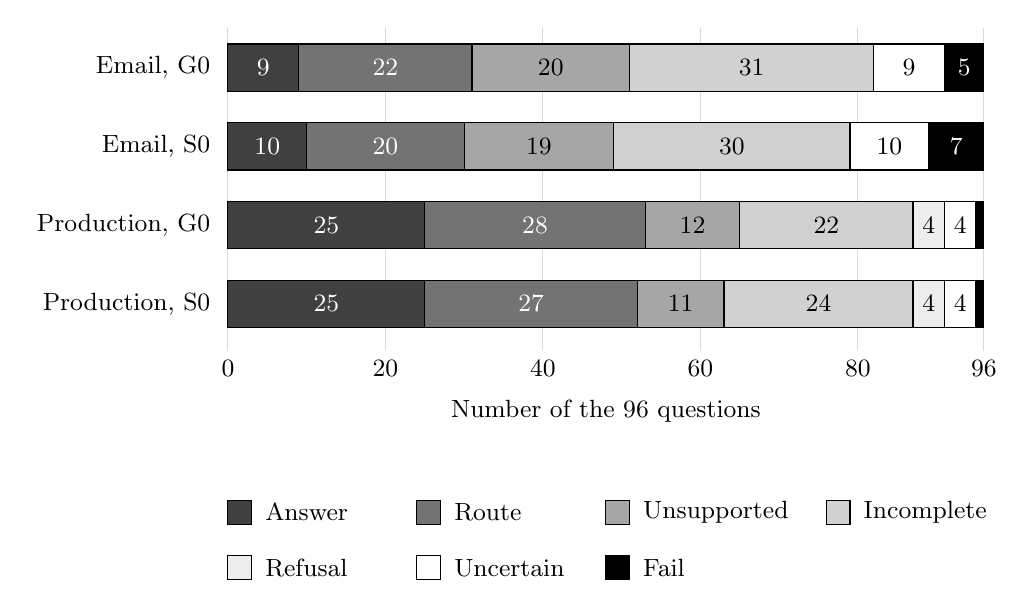
\begin{tikzpicture}[x=0.1cm,y=1cm,font=\small]
  \foreach \p in {0,20,40,60,80,96} {
    \draw[black!15] (\p,0.5) -- (\p,-3.6);
    \node[below] at (\p,-3.6) {\p};
  }
  \node[below] at (48,-4.1) {Number of the 96 questions};
  \node[left] at (-1,0) {Email, G0};
  \node[left] at (-1,-1) {Email, S0};
  \node[left] at (-1,-2) {Production, G0};
  \node[left] at (-1,-3) {Production, S0};
  % cumulative boundaries: Answer, Route, Unsup., Incomp., Abstain, Uncert., Fail
  \foreach \y/\pa/\pb/\pc/\pd/\pe/\pf/\pg/\ph in {
    0/0/9/31/51/82/82/91/96,
    -1/0/10/30/49/79/79/89/96,
    -2/0/25/53/65/87/91/95/96,
    -3/0/25/52/63/87/91/95/96} {
    \fill[black!75] (\pa,\y-0.3) rectangle (\pb,\y+0.3);
    \fill[black!55] (\pb,\y-0.3) rectangle (\pc,\y+0.3);
    \fill[black!35] (\pc,\y-0.3) rectangle (\pd,\y+0.3);
    \fill[black!18] (\pd,\y-0.3) rectangle (\pe,\y+0.3);
    \fill[black!7] (\pe,\y-0.3) rectangle (\pf,\y+0.3);
    \fill[white] (\pf,\y-0.3) rectangle (\pg,\y+0.3);
    \fill[black] (\pg,\y-0.3) rectangle (\ph,\y+0.3);
    \draw (\pa,\y-0.3) rectangle (\ph,\y+0.3);
    \foreach \u in {\pb,\pc,\pd,\pe,\pf,\pg} { \draw (\u,\y-0.3) -- (\u,\y+0.3); }
    \ifnum\numexpr\pb-\pa\relax>2 \node[text=white] at ({(\pa+\pb)/2},\y) {\the\numexpr\pb-\pa\relax}; \fi
    \ifnum\numexpr\pc-\pb\relax>2 \node[text=white] at ({(\pb+\pc)/2},\y) {\the\numexpr\pc-\pb\relax}; \fi
    \ifnum\numexpr\pd-\pc\relax>2 \node at ({(\pc+\pd)/2},\y) {\the\numexpr\pd-\pc\relax}; \fi
    \ifnum\numexpr\pe-\pd\relax>2 \node at ({(\pd+\pe)/2},\y) {\the\numexpr\pe-\pd\relax}; \fi
    \ifnum\numexpr\pf-\pe\relax>2 \node at ({(\pe+\pf)/2},\y) {\the\numexpr\pf-\pe\relax}; \fi
    \ifnum\numexpr\pg-\pf\relax>2 \node at ({(\pf+\pg)/2},\y) {\the\numexpr\pg-\pf\relax}; \fi
    \ifnum\numexpr\ph-\pg\relax>2 \node[text=white] at ({(\pg+\ph)/2},\y) {\the\numexpr\ph-\pg\relax}; \fi
  }
  % legend
  \foreach \x/\fl/\tx in {0/black!75/Answer, 24/black!55/Route, 48/black!35/Unsupported, 76/black!18/Incomplete} {
    \fill[\fl,draw=black] (\x,-5.8) rectangle (\x+3,-5.5);
    \node[right] at (\x+3.5,-5.65) {\tx};
  }
  \foreach \x/\fl/\tx in {0/black!7/Refusal, 24/white/Uncertain, 48/black/Fail} {
    \fill[\fl,draw=black] (\x,-6.5) rectangle (\x+3,-6.2);
    \node[right] at (\x+3.5,-6.35) {\tx};
  }
\end{tikzpicture}
\caption[Outcome categories of the AI judge for G0 and S0 in each sample, out of 96 questions]{Outcome categories of the AI judge for G0 and S0 in each sample, out of 96 questions. Answer is a supported answer and Route is useful routing. Together they count as assistance. Segments of one or two questions are not labeled. Counts for all four policies are in Table~\ref{tab:luna-outcomes}.}
\label{fig:outcome-bars}
\end{figure}
